\documentclass[10pt]{article}

\usepackage{amsmath,amsfonts,amssymb}
\usepackage{graphicx}  % For including pictures
\usepackage{tikz}  % For plotting
\usepackage{color}  % For changing text color
\usepackage{cancel}  % For crossed-out math
\usepackage{ulem}  % For strikethrough

% Tailor paper size and margins
\usepackage[a4paper, top=2.5cm, bottom=2.5cm, left=2.2cm, right=2.2cm]{geometry}
%\usepackage[margin=0.8in]{geometry}
% More margin customization
%\addtolength{\oddsidemargin}{-.875in}
%\addtolength{\evensidemargin}{-.875in}
%\addtolength{\textwidth}{1.75in}
%\addtolength{\topmargin}{-.875in}
%\addtolength{\textheight}{1.75in}

\setlength{\parskip}{1pt}
%\setlength{\parindent}{0pt}  % Uncomment to remove all indentation from paragraphs

\linespread{1.5}
%\renewcommand{\baselinestretch}{1.5}

\numberwithin{equation}{section}  % Include section in equation numbering

\title{Lin's Notes on the Theory of Machine Learning}
\author{Lin Xu}

\begin{document}

\maketitle

\vspace{10mm}

\begin{abstract}
The holy grail of machine learning is finding an in-sample estimate of the out-of-sample error. To achieve this goal, we shall ask ourselves two questions:
\begin{enumerate}
    \item Is in-sample error, $E_\mathrm{in}$ small enough?
    \item Is out-of-sample error, $E_\mathrm{out}$ close enough to $E_\mathrm{in}$?
\end{enumerate}

Apparently, these two aims don't get along with each other. Armed with a more complex model, we are almost assured to have a lower $E_\mathrm{in}$. But a complex model might also lead to a larger $E_\mathrm{out}$ provided that the number of records in the training set is not sufficient enough, which is known as the overfitting issue. This note will develop the logic to pin this relationship concretely by drawing heavily on the concepts and notes taken in the Learning from Data course.

Also note that this article only focuses on Supervised Learning.
\end{abstract}


\section{Feasibility of Learning}

The essence of machine learning can be summarized into the three bullet points below:
\begin{itemize}
    \item A pattern exists;
    \item We cannot pin it down mathematically;
    \item We have data on it.
\end{itemize}
If all the three criteria are met, we are in business with machine learning. The next question is how to do machine learning. Figure \ref{fig:learndiag} is a diagram of the procedures. Professor Abu-Mostafa spent several lectures to obtain this diagram by starting from a simplified version and adding more ingredients to it gradually. Here I saved the endeavor and just present the final version.
\begin{figure}
    \center{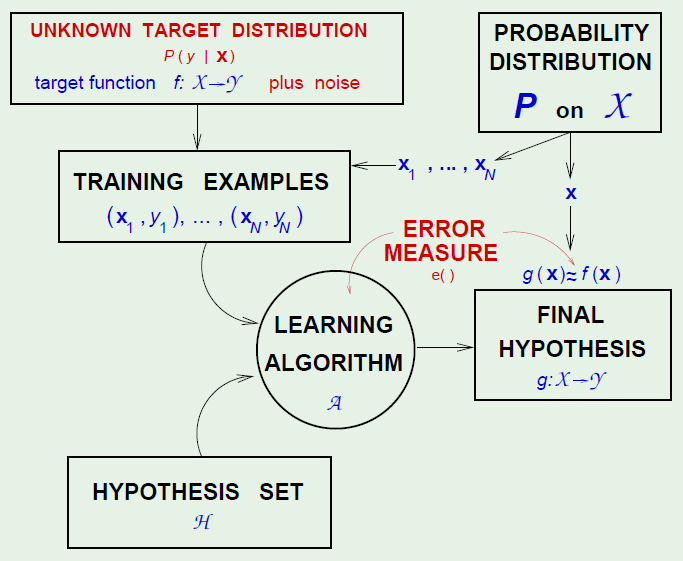
\includegraphics[width=0.6\linewidth]{figure/learning_diagram.png}}
    \caption{The Learning Diagram}\label{fig:learndiag}
\end{figure}

Apparently, the core procedure is learning from sample. We then need to justify that learning from sample is feasible. Hoeffding's inequality provides a theoretical support. It describes the relation between in-sample and out-of-sample error in probabilistic terms. Provided a certain hypothesis $h$,
\begin{equation}\label{eq:hoeffdingtest}
    \mathbb{P}[\vert E_\mathrm{in}(h)-E_\mathrm{out}(h)\vert > \epsilon] \leq 2e^{-2\epsilon^2N}
\end{equation}
where $\epsilon$ is the error term, $N$ is the sample size. One advantage of Hoeffding's inequality is that the bound does not depend on the learning target, which enables it to be applied to all kinds of learning problems.

Note that Inequality \eqref{eq:hoeffdingtest} is an expression of testing, that is, it only works for a given hypothesis. For training we would like to pick the ``best-fitting in-sample" hypothesis in a \textbf{hypothesis set} $\mathcal{H}$. If $\mathcal{H}$ is large enough, it's very likely for us to get a hypothesis with tiny in-sample error. But does it provide a good estimate of out-of-sample error? The answer is most likely NO! We are probably just lucky enough to find one fitting the sample itself very well. Think of $p$-value (the probability of obtaining the observed sample results when the null hypothesis is actually true) as an analogy. If you do an experiment as many times as possible, you will eventually get it right!

Intuitively, we shall involve the size of $\mathcal{H}$ (or equivalently model complexity) in the inequality as a factor of cost. Given a hypothesis set $\mathcal{H}$, in the most conservative case, the experiment for each hypothesis in the set is independent. Hence, we can do a simple summation to obtain the inequality of the hypothesis set (\textit{i.e.} the expression of training),
\begin{equation}\label{eq:hoeffdingtrain}
    \mathbb{P}[\vert E_\mathrm{in}(g)-E_\mathrm{out}(g)\vert > \epsilon] \leq 2\textcolor{red}{M}e^{-2\epsilon^2N}
\end{equation}
where $g$ is a hypothesis picked from $\mathcal{H}$. We will establish later on that relaxing the independence assumption will make learning feasible.

The intuition behind Inequality \eqref{eq:hoeffdingtrain} is that the more hypotheses you try the higher the probability of getting one with very small in-sample error is. $M$ is the price of going through all those hypotheses, and thus, complexity of the hypothesis set $\mathcal{H}$ means a larger $M$. If we have a more complex model, we will fit better in-sample but need more examples (a bigger $N$) to negate the large $M$ in order to satisfy the inequality. The inequality as it is does not offer too much hope since $M$ is often infinity in practice! In the next section, we will introduce a more accurate measure of model complexity to replace $M$ so that the inequality becomes a sound basis for learning feasibility.


\section{Measure of Model Complexity}

From discussion in the previous section, we figured that Inequality \eqref{eq:hoeffdingtrain} is not good enough because $M$ is not a proper measure of model complexity. In order to establish an appropriate measure of model complexity, first we need to introduce the concept of dichotomy. Dichotomy is a partition of a whole (or a set) into two parts (subsets) that are:
\begin{itemize}
    \item jointly exhaustive: everything must belong to one part or the other, and
    \item mutually exclusive: nothing can belong simultaneously to both parts.
\end{itemize}
Such a partition is also frequently called a bipartition.

To better illustrate this concept, let's look at the example of 2-D perceptron. With $N$ points in a two-dimensional space, how many dichotomies can we have at most? The answer is $2^N$, easy enough. However, if we want to do the partition with a straight line, we won't be able to get all $2^N$ dichotomies. And the reason is obvious, that is, our model, straight line, is too simple to capture all possible dichotomies. Hence, although the $M$ is infinite in this case, it doesn't necessarily mean our model is extremely complex. And the uncomplexity is reflected by the limited number of dichotomies the model can achieve. Good news! So we can establish a measure of model complexity based on how many dichotomies the model can get most.

Let's define a measure called Growth Function,
\begin{equation}
    m_\mathcal{H}(N) = \max_{x_1, \dots, x_N \in \mathcal{X}} \vert \mathcal{H}(x_1, \dots, x_N)\vert
\end{equation}
which counts the most dichotomies on any $N$ points for a given model or hypothesis set $\mathcal{H}$. And we can argue that the complexity of a model or hypothesis set can be measured by the growth function.

Note that the growth function must satisfy $m_\mathcal{H}(N) \leq 2^N$ since $2^N$ is the maximum number of dichotomies a data set of size $N$ can possibly have. A fair question is: when does the equality hold? Back to the perceptron example, we can easily show that $m_\mathcal{H}(N) = 2^N$ for $N \leq 3$. If a model (hypothesis set $\mathcal{H}$) can capture all possible dichotomies of a data set, we say that the model or $\mathcal{H}$ can ``shatter" the data set. Thus, a 2-D perceptron can shatter a data set with 3 points at most. Intuitively, a more complex model should be able to ``shatter" data set with more points.

Now we are ready to introduce the key notion of this section -- break point. The \textbf{break point} of a model or hypothesis set $\mathcal{H}$ is the \textcolor{red}{smallest} $k$ where no data set of size $k$ can be shattered by $\mathcal{H}$.

Regarding this very important notion, we need to clarify some potential confusions. First, it's obvious but not trivial to conclude that if $\mathcal{H}$ can shatter no data set of size $k$, it won't be able to shatter any data set of size larger than $k$. Hence, the break point is a critical threshold. Second, an $\mathcal{H}$ with break point $k$ may not be able to shatter all data sets of size smaller than $k$. As we know that the break point for the 2-D perceptron is 4. However, given 3 points on a straight line, the perceptron cannot capture the dichotomy with two points on the sides as one group and the one in the middle as another. But as long as it manages to get all possible combinations for one data set with 3 points, its break point is larger than 3.\footnote{Possible homework: try figure out the break point for different models.}

Both growth function and break point are extremely important measure of model complexity. They are useful in different ways. Growth function is introduced to replace $M$ in the Hoeffding's inequality for training. It must depend on the data set because it measures the cost of training on the data set given certain model. Break point on the other hand, depends only on the model itself. It's useful when we want to determine what model to use given a data set. We would't like a model with large break point if we have a small data set. Think of an extreme case when a model manages to get all possible dichotomies for a data set. It's almost for sure overfitting. Third, a model with infinite break point have $m_\mathcal{H}(N) = 2^N$ for any $N$. Such model is not suitable for learning as it can always fit the sample set perfectly and cannot be generalized to out-of-sample set.

We've been saying that we want to use growth function $m_\mathcal{H}(N)$ to replace $M$. Question is can we really do that? We also need to figure out the form of $m_\mathcal{H}(N)$. It doesn't have to be an explicit expression as long as we can prove that the exponential $e^{-2\epsilon^2N}$ will eventually manage to bring the RHS of Inequality \eqref{eq:hoeffdingtrain} down given a large $N$, so that learning using the hypothesis set $\mathcal{H}$ becomes feasible given enough number of data points. An educated guess is that $m_\mathcal{H}(N)$ (of course $\mathcal{H}$ must have a finite break point) is polynomial. But is it a valid guess? In the next section, we will answer these two questions.


\section{Theory of Generalization}

To summarize, to be able to generalize and show that learning from data is feasible, we need to have two things in place:
\begin{enumerate}
    \item proof that $m_\mathcal{H}(N)$ is polynomial,
    \item proof that $m_\mathcal{H}(N)$ can replace $M$.
\end{enumerate}
Once you have them, negative exponential in Hoeffding's inequality will eventually triumph.

First, let's prove that $m_\mathcal{H}(N)$ is polynomial. Let $B(N,k)$ be the maximum number of dichotomies on $N$ points, with break point $k$.

Replacing $M$ with $m_h(N)$ results in VC inequality formula below, which is arguably the most important equation in machine learning. The inequality helps us to narrow the union bound into Vapnik-Chervonenkis (VC) inequality:
\begin{equation}\label{eq:vc}
    \mathbb{P}[\vert E_{in}(g)-E_{out}(g)\vert > \epsilon] \leq 2m_\mathcal{H}(2N)e^{-1/8\epsilon^2N}
\end{equation}

If there is a break-point for hypothesis set, we are in business. You can have a $g$ such that $E_{in}$ track $E_{out}$ well given large enough sample size. Note that what we talked about is independent of ``target function". This is important, because we do not know and will not know the ``target function".

In the next section, we will discuss in detail the core notion of the whole article -- VC Dimension! The VC dimension of a model in simple terms corresponds to the number of points it can shatter, hence the complexity of the model.


\section{The VC Dimension}

The VC dimension of a hypothesis set $\mathcal{H}$, denoted by $d_{VC}(\mathcal{H})$, is the largest value of $N$ for which $m_\mathcal{H}(N)=2^N$, \textit{i.e.} ``the most points $\mathcal{H}$ can shatter".
If $d_{VC}$ is finite, $g\in H$ will generalize. Note that this is a probabilistic statement in the form of VC Inequality.

In general, think of $d_{VC}$ as the effective number of parameters that you can dial in to get to all dichotomies. Therefore, the VC dimension is a very criterion of choosing the model with proper complexity.

Transform VC inequality into generalization bound:
\begin{equation}
    \mathbb{P}[\vert E_{out}-E_{in} \vert \leq \Omega(N,\mathcal{H},\delta)]\geq 1-\delta
\end{equation}
where $\Omega$ defines how well the model is generalized, and specifically
\begin{equation}
    \Omega(N,\mathcal{H},\delta)=\sqrt{\frac{8}{N}\ln\frac{4m_\mathcal{H}(2N)}{\delta}}
\end{equation}
where $N$ is the sample size; $\mathcal{H}$ is the hypothesis set with certain complexity; $\delta$ is probability of error in VC bound.

We can conclude the following:
\begin{itemize}
    \item A more complex model is better for $E_{in}$ (this is always true) but bad for $\Omega$ and hence for $E_{out}$.
	\item If you want the probability of error to be lower, you will need a higher $N$.
	\item A larger $N$ narrows the gap between $E_{in}$ and $E_{out}$.
\end{itemize}
